\chapter{Simulation}
\label{chapter:simulation}

After introducing the general underlying ideas and topics associated with the issue of this work, I will now explain the simulation, which is the core topic of this work and go further into detail. 
\cite{lipman2009language} argued "that we cannot explain the prevalence of vague terms in
natural language without a model of bounded rationality which is significantly different from anything in the existing literature". I will argue with the results of the simulation, that the prevalence of vague terms can be explained with the RSA model, which is a model of bounded rationality.
The human ability of recursive reasoning about the mind state of the communication partner might enable us to understand vague terms and infer correct world states after hearing them, in order to communicate efficiently.

\section{General assumptions and procedure}
A communication situation which is to be modeled here was already introduced in chapter 2, but I will again shortly recap the procedure of the sender-receiver-game:\\

There are two players/agents, a speaker $S$ and a listener $L$. $S$ observes a world state $w$, randomly drawn from a distribution function $Pr(w)$ (= world prior). In this case, $w$ is to be interpreted as the height of a person. Then, $S$ chooses a message $m$ from a set of alternatives $M$, to describe the observed $w$ to $L$, who cannot observe $w$ directly. Dependent on the observed message $m$, $L$ chooses an action $a$, which in this case is simply guessing the intended world state $w$. The probability, that listener $L$ infers the correct height is calculated for computing an "expected utility (EU)" value (more on EU in section \ref{sec:EU}). This serves as a measure of communicative success and is later used for evaluating the simulation results, in an examination of evolutionary stable strategies. A schematic figure of a communication situation is given in Fig.\ref{figure:procedure}.\\

Each agent is of a certain \textit{type}. These types differ in their belief about the actual semantics of a gradable adjective like \textit{tall}, more specifically in their belief about the underlying threshold, after which to use \textit{tall} (e.g. crisp vs. vague threshold). The next section should clarify the actual semantics of the possible utterances by showing an implementation of a lexicon that uses the meaning function defined in chapter 3. After that, I will make further assumptions about the world prior distribution from which the world states for the speaker's observation are drawn. At the end of this chapter, the actual simulation is presented and explained, including the quantitative measure of communicative success (EU).
\begin{figure}
 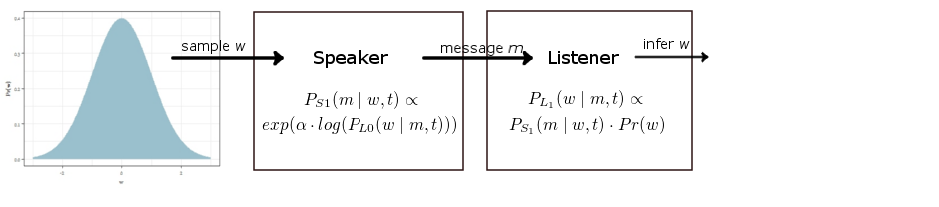
\includegraphics[scale=0.7]{procedure.png}
 \caption{Schematic presentation of a communication situation.}
 \label{figure:procedure}
\end{figure}
\section{Vague meaning in the lexicon}
How is a vague word like \textit{tall} to be interpreted? How can we quantitatively capture the vagueness in a semantic description in a lexicon? As introduced in chapter \ref{chapter:rsa-model}, I implemented the meaning as a degree to which an utterance is true, given the utterance and the \textit{type} of an agent, as a function over world states.\\

A "truth-function", for each possible utterance has to be implemented, in order to form a lexicon that serves as a rudimentary basis for language understanding and language use. The message set of alternatives considered here is $M = \{$\textit{short}, \textit{tall}, \textit{not-short}, \textit{not-tall}$\}$. Lexical antonyms like \textit{short} and \textit{tall} are treated differently than the respective logical negations \textit{not-short} and \textit{not-tall}. The behaviour of negated vague terms is not trivial, but has been empirically studied and quantitatively modeled by \cite{tesslernot}. Similar results can be replicated in this simulation, with respect to the use and understanding of the negation of vague terms and their antonyms.\\

One possibility for expressing meaning would be to consider different thresholds for \textit{tall} and \textit{short} as well as the interpretation of "not" as logical negation. In the following description, $w$ is some world state, i.e. a height value:
\begin{align*}
\text{"tall"} \rightarrow& \,\, w > \theta_{tall}\\ 
\text{"not-tall"} \rightarrow& \, \neg (w > \theta_{tall})\\
\text{"short"} \rightarrow& \,\, w < \theta_{short}\\
\text{"not-short"} \rightarrow& \, \neg (w < \theta_{short})\\
\end{align*}
Such an implementation of a meaning function maps a world state to either true or false (one or zero), like in Figure \ref{subfig:cdf-crisp}. For adding vagueness to the semantics, the threshold $\theta_{tall}$ is not given by a crisp number, but a Gaussian probability distribution over possible values for $\theta$. Language use changes over time, so it seems more natural to assume that the same world state might lead to different message choices of a speaker at different points in time, due to vague semantics. It also seems natural to assume that the degree to which the word \textit{tall} is true should increase gradually with increasing height $w$. This behavior is modeled well by a cumulative distribution function $\Phi$ over the prior expectation about $\theta$, as introduced in chapter \ref{chapter:rsa-model}. The concrete semantics for the utterances \textit{tall} and its negation are given below. The semantics for \textit{short} and its negation are analogous.
\begin{align*}
\llbracket \textsf{"tall"} \rrbracket^{w, \mu,\sigma} &= \Phi(P(\theta_{tall} \mid \mu, \sigma))(w)\\
\llbracket \textsf{"not-tall"}  \rrbracket^{w, \mu,\sigma} &= 1 - \Phi(P(\theta_{tall} \mid \mu, \sigma))(w)
\end{align*}
Little uncertainty about the value of the threshold is described by a small value for $\sigma$ in the threshold prior, resulting in a crisp meaning, while a bigger $\sigma$ will lead to a more vague interpretation. A visualization of such vague literal semantics can be viewed in Figure \ref{figure:litsemantics}.
As a natural consequence of this degree semantics, borderline cases are modeled correctly in the sense that it is not deterministic whether \textit{tall} is true or not for a certain $w$, but it is true to a certain degree.
\begin{figure}
 \centering
 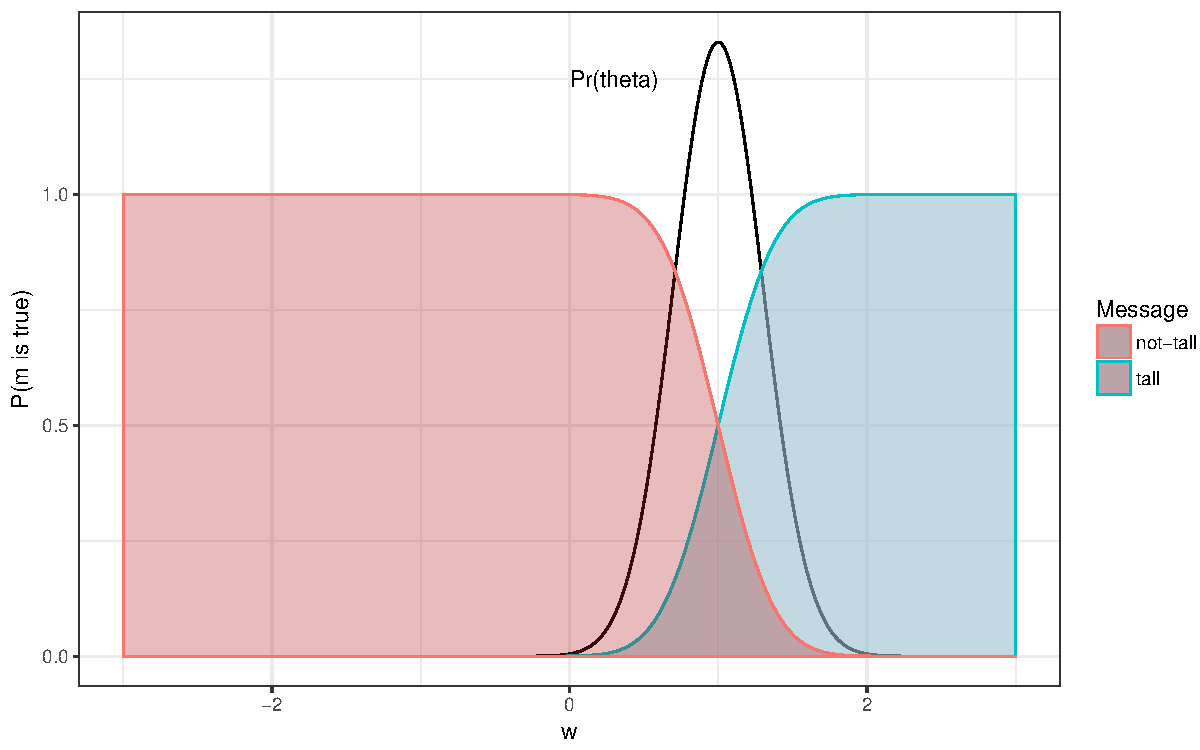
\includegraphics[scale=0.6]{lit_tall_vague.pdf}
 \caption{Literal vague meaning of \textit{tall} and \textit{not-tall}. The distributions for \textit{short} and \textit{not-short} look similar.}
 \label{figure:litsemantics}
\end{figure}

\section{World prior}

The chosen world prior distribution $Pr(w)$ of heights is a standard normal distribution with mean $\mu = 0$ and $\sigma = 1$. With this normalized choice, it is possible for interpretation to move this distribution to any scale of interest, like e.g. size of people, measured in m. 
It allows very general interpretations and brings the advantage of not having to specify a scale that is relevant, i.e. a comparison class.  It seems natural in the present model to capture the effect of a comparison class as an effect of the world prior choice. While comparison class inferences has been studied in other works, I will keep this factor standardized in this simulation.\\

Gradable adjectives seem to be interpreted in a "norm-related" way (Fara 2000), so that \textit{tall} would mean "taller than the norm", while the norm is dependent on a comparison class. This allows for symmetric behaviour of the thresholds for \textit{short} and \textit{tall}, because \textit{short} would also mean "shorter than the norm". It is considered that a deviation from the norm in the positive direction that counts as \textit{tall}, is the same deviation in the negative direction for counting as \textit{short}. From this assumption follows $\theta_{short} = -\theta_{tall}$.

\section{Goal of simulation}

An agent's type comprises a certain semantics. I want to investigate which semantics is optimal if agents behave rationally, according to the RSA model.
For measuring communicative success of two agent types, the probability that the speaker might choose a specific message $m$ for a specific world state $w$ is calculated, as well as the probability that the listener does "understand" this utterance, in the sense that the inferred world state equals $w$.\\

In the simulation, the "conversations" are simulated on all possible world states as well as all possible utterances. The overall expected utility (EU) is calculated for a given speaker- and listener type (more on the EU in the next section).
This calculation is performed on all possible pairs of all possible types of agents, to investigate which agent strategies perform well and which do not. 

\section{Expected Utility}
\label{sec:EU}
The expected utility (EU) of two agent types $t_1$ and $t_2$ quantifies the communicative success of these two agents playing the sender-receiver game repeatedly. $t_1$ and $t_2$ are considered to be the speaker and listener at half of the time respectively. To obtain $EU(t_1, t_2)$, I take into account each possible state $w$ as well as each possible utterance the speaker could make to describe the respective state. The EU of two agents is the probability that speaker $S_1$ would choose message $m$ and listener $L_1$ would infer the right world state $w$ after seeing $m$. This is summed over all possible world states and all possible messages, weighted with their prior probabilities. The message prior is uniformly distributed, therefore this term is omitted in the following formula:
\begin{align}
EU(t_1, t_2) = \sum \limits_{w} \sum \limits_{m} 0.5 \cdot \big[ &P_{S_1}(m\,|\,w ,\, t_1) \cdot P_{L_1}(w \mid m ,\, t_2) \cdot Pr(w) + \\
&P_{S_1}(m \mid w ,\, t_2) \cdot P_{L_1}(w \mid m ,\, t_1) \cdot Pr(w) \big] \nonumber
\end{align}
The simulation consists of an EU-computation for all possible agent pairs, for examining the effectiveness of different strategies/semantics. To evaluate which strategies perform best, I search for evolutionary stable strategies (ESS, this concept has been introduced in chapter \ref{chapter:vagueness-pragmatics}). Which agent types are used in the simulation is presented in the next section.

\section{Simulation set-up}

In the simulation, the types are combined from the following parameter spaces:
\begin{align*}
\mu &\sim \{ 0, 0.1, 0.2, ... , 2.0 \} \\
\sigma &\sim \{ 0.001, 0.1, 0.2, ... , 2.0 \} \\
\alpha &\sim \{ 1, 5, 10, 50, 100 \}
\end{align*}
All of these possible parameters are combined into a set of 2000 possible agent types in total, consisting of all possible combinations of the parameters $\mu$, $\sigma$ and $\alpha$. The set of $\mu$'s and $\sigma$'s could be chosen according to a comparison class, if this is desired. The results would look quantitatively different but qualitatively the same.
Example types would look like this: $t_1=[\mu=1.2, \sigma = 0.4, \alpha=5]$, $t_2=[\mu = 0.8, \sigma = 0.1, \alpha=50]$. A visualization of possible listener strategies is given in Fig.\ref{figure:L1-posterior}. It shows probability distributions over 
% message choices, $P(m | w, type)$ on the speaker side or 
interpretation choices, $P(w \mid m, type)$ on the listener side. In the following chapter the results of the simulation are presented, i.e. the EU-values for any agent pair as well as ESS. 